\chapter{Deep Learning approach for the Food Image Classification}
\lhead{\emph{Deep Learning approach for the Food Image Classification}}

In this chapter short introduction to deep learning is provided. Then the library used for building deep learning classifiers is described. Finally, deep learning models are constructed, and their performance is evaluated.


\section{Short Introduction To Deep Learning}

Deep learning is often regarded as an exciting and new technology. In reality, the field dates back to 1940s. The earliest predecessors of modern deep learning were simple linear models motivated from a neuroscientific perspective. These models were designed to take a set of n input values \(x_1,...,x_n\) and associate them with an output \(y\). These models would learn a set of weights \(w_1,...,w_n \) and compute their output \(f(x,w)=x_1 w_1+...+x_n w_n\) \cite{Goodfellow-et-al-2017}. The same function is used in today’s deep neural networks. A deep neural network contains a set of these functions connected in a way where the output of the previous function is the input to the next function. The result of \(f(x,w)\) is then passed through the non-linear activation function to make the result non-linear. The most commonly used activation function today is a Rectified linear unit(ReLU). The function can be mathematically described as \(f(x)=max(0,x)\) which means that it always outputs 0 for values less than 0 and \(x\) for values greater than 0. Illustration of this is shown in \autoref{fig:relu}. Neural networks using this function usually converge faster than networks using a different activation function \citep{relu}.

\begin{figure}[h]
\centering
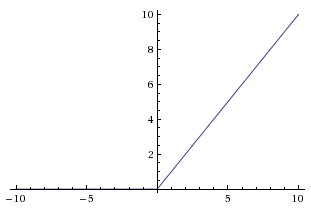
\includegraphics[width=0.5\textwidth]{Figures/relu.jpeg}
\caption{The ReLU activation function \citep{231nn}}
\label{fig:relu}
\end{figure}


\section{Introduction to TensorFlow}

TensorFlow is an interface for expressing machine learning algorithms and an implementation for executing such algorithms. A computation expressed using TensorFlow can be executed with little or no change on a wide variety of systems, ranging from mobile devices such as phones and tablets up to large-scale distributed systems and thousands of computational devices such as GPU cards \cite{abadi2016tensorflow}. The system is flexible and can be used to express a wide variety of algorithms for deep neural network models. It has been used for conducting research and for deploying machine learning systems into production across more than a dozen areas of computer science and other fields \cite{abadi2016tensorflow}. Computations in TensorFlow are described in a directed graph. First, all operations are listed and added to the graph, then a TensorFlow session is called and executes the operations in a graph. An example of a TensorFlow program that adds two scalars and computes the result can be seen in \autoref{fig:sess}. Executing tf.add(5, 5) creates a node in the computational graph with 5 and 5 as the input values. The result of the add operation is only computed when a TensorFlow session is created. 

It was decided to use TensorFlow to construct deep neural network models for food image classification because this library is fast and efficient. It is used by many deep learning researchers. However, because TensorFlow was created primary for conducting deep learning research, algorithms provided in this library are low level and require additional implementations to make them work on a particular dataset.

Because of the complexity and a low-level implementation, it was a very challenging task to learn and understand how to use TensorFlow correctly. It was firstly tried to implement deep learning models for the default datasets provided in the TensorFlow library, to get familiar with TensorFlow. After spending a significant amount of time studying deep learning methods and writing implementations of deep learning algorithms, steps needed to train a neural network model with TensorFlow were eventually discovered. However, before training the models the dataset, needed to be transformed into a format supported by TensorFlow. 

\begin{figure}[h]
\centering
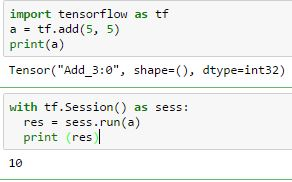
\includegraphics[width=0.5\textwidth]{Figures/4/sess.jpg}
\caption{Example of a TensorFlow program that computes the result of adding two scalars}
\label{fig:sess}
\end{figure}

\section{Transformation of the Dataset For Using It with TensorFlow}

Before using the food image dataset, additional preprocessing techniques needed to be applied. The class labels of this dataset were represented by strings e.g.: "Pizza". Non-numerical class names cannot be used when computing a distance function or other functions that are used in machine learning. Therefore, class labels had to be transformed using one-hot encoding. One-hot encoding converts every class name into a vector which has the length equal to the number of classes. For every class, one element in a vector is set to one while other elements are set to zeros. The previously used Sckit-learn library encoded the labels automatically, but in TensorFlow this task has to be done manually.

To one-hot encode, the labels of the dataset were first transformed into numeric values from 1 to 4. After that, a vector equal to the number of classes was created, and numeric values were transformed to one hot encoded values \autoref{table:oh}. After the transformation of the dataset had been done, it was possible to use it for training deep learning networks with TensorFlow.


\begin{table}[h]
\begin{center}
\begin{tabular}{ |c|c|c| } 
 \hline
 Label &   Numeric label & One-hot Encoded label  \\   \hline
 Fish and Chips    &   1  &   [0, 0, 0,1]  \\
            Pizza   &   2 &    [0, 0, 1,0]    \\
            Salad    &   3 &    [0, 1, 0,0]    \\
Vanilla Ice Cream     &  4  &   [1, 0, 0,0]    \\ 
 \hline
\end{tabular}
\caption{Applying labels encoding to the dataset}
\label{table:oh}
\end{center}
\end{table}


\section{Linear Classifier in TensorFlow}
It was decided to construct linear classifier as a first TensorFlow classification model. This classifier was chosen because it is very simple compared to other neural networks. Furthermore, a linear classifier is a building block of every deep learning model, so it was  important to understand it well before building more complex classification models

\subsection{Introduction to a Linear Classifier}
 Linear classifier can be described as a function \(y = w\times X\). In a case of image classification, \(y\) is a class of an image, \(X\) is a vector of pixels of an image and  \(w\) is a vector of weights that are associated with each pixel. The fact that each pixel has a separate weight associated with it allows this classifier to learn the important areas of pictures in each class automatically. The classifier can calculate which parts of the image have a large influence when classifying an image and make the weights of these pixels large. The weight of pixels that have no or tiny impact to the class of a picture can be set to values close to zero.

\subsection{Training  of  the Linear Classifier}
To begin training the model, the weights were initialized with random values from a generated normal distribution with 0.01 standard deviation. After the weights had been initialized, the classifier tried to classify the data with the initialized weights. Then, the error function was calculated, and the weights were updated to the new values that decreased the error function. The update rate value was controlled by a learning rate. The learning rate that was used to train this model was 0.005. To perform the weight optimisation a gradient descent and Adam optimizer was tried.

Gradient descent is an algorithm that tries to minimise the training lost, and  the Adam optimizer is a gradient descent optimisation algorithm \cite{adam}. Adam works well in practice and compares favourably to other optimisation methods. The advantage of Adam optimizer is that it can start optimising weights with a high learning rate and then automatically decreases it as the algorithm continues to train. Consequently, Adam optimizer can find the optimal weights faster than a gradient descent.

It is possible to train an optimisation algorithm on the full dataset or use batch optimisation. For using batch optimisation,  the training dataset has to be split into batches of equal size. Then, optimisation algorithm runs on the one batch of the dataset, updates the weights of the full dataset, and uses a different batch for optimising the weights again. The advantage of using a full dataset for weights optimisation is that more data usually leads to a better weight optimisation. However, running this algorithm can take a very long time. Usually, batch optimisation is faster and can achieve similar results.

To do a batch optimisation, the food image dataset was split into 54 batches containing 87 food images each. From all trained linear classification models the classifier using the Adam Optimizer with 0.05 learning rate and the batch optimisation performed the best. It achieved 51.53 percent accuracy. A table of classifiers tested and their performance can be seen in \autoref{table:linear}. To be able to use these models without having to retrain them, they were saved to a disk.


\subsection{Results}
From the results table, it can be observed that optimisation on the full dataset performed very poorly compared to the batch optimisation method.  This happened because the weights on batch optimisation were updated 56 times more often. It can also be observed that Adam Optimizer was a better optimisation algorithm than a gradient descent. It performed 7.09 percent better.

To conclude, despite the fact that a linear classifier is such a simple algorithm, it was possible to optimise it to classify the images with a reasonable accuracy.

\begin{table}[h]
\begin{center}
\begin{tabular}{ |c|c|c|c| } 
 \hline
 Learning Rate &   Optimization Function & Batch Size & Classification Accuracy \\   \hline
0.005    &   Adam Optimizer  &  85  & 51.53\% \\
0.005    &   Adam Optimizer  &  full dataset  & 26.00\% \\
0.005    &   Gradient Descent Optimizer  &  85  & 44.44\% \\ 
 \hline
\end{tabular}
\caption{The influence of optimization function and its hyperparameters to the classification accuracy}
\label{table:linear}
\end{center}
\end{table}

\section{Multi-layer Neural Network in TensorFlow}

After building a linear classifier, it was decided to expand it to build a deep neural network, which could learn a better representation of the data. The structure of the model was designed in the following way: 30.000 neurons in the input layer, two hidden layers containing 256 neurons each and a final layer containing four neurons that map to the four image classes.A ReLu activation function was used in hidden layers 1 and 2  to introduce a non-linearity to the network. 


After starting to train the model, it was observed that after a couple of training epochs the training accuracy stopped improving and stayed the same during all the duration of training. When tested on the test dataset, the classifier classified the food images with only 24 percent accuracy, which was even worse than a random guessing. It was, though that the problem was with the learning rate being too high. However, decreasing the learning rate did not solve the problem. Then, it was tried to change the structure of the network by changing the number of layers in the network and number of neurons in each layer, but modifying the structure did not solve the problem either. Various sets of different hyper-parameters were tried to fix the network, but nothing seemed to work. It was finally noticed that the problem was caused by a wrong activation function used in a final layer. TensorFlow library did not provide any warning about the error making it hard to detect the problem. 

After fixing the error, the classifier was trained using the Adam optimizer with a learning rate of 0.0001. When tested this classifier achieved 56.32 percent accuracy. It was noticed that during the training of this classifier, the cost function decreased slowly. Because of that, it was decided to increase the learning rate to 0.001. However, this learning rate seemed to be too large, and the classifier accuracy decreased to 47.50 percent. Then 0.0005 learning rate was used. The network trained with this learning rate classified the test data with 54.02 percent accuracy. After experimenting the different learning rates, it was concluded that  0.0001 was the optimal learning rate for this neural network.

Finally, it was decided to try to increase the number of layers in this neural network. It was expected that a deeper network would be able to learn a better representation of the dataset. Five layer neural network model with four hidden layers that have 256, 256,256 and 128 neurons classified the test dataset with 56.32 accuracy. This accuracy was the same as achieved with a three-layer neural network. It was tried to improve accuracy by changing the number of neurons in different layers. The neural network that had fewer neurons in the final hidden layer performed a bit better, but no other significant improvements for classifying the test dataset were noticed. A full table of multilayer classifiers that were trained and their performance can be seen in \autoref{table:multi}.

\begin{table}[h]
\begin{center}
 %\setlength\tabcolsep{2pt}
\begin{tabular}{ |c|c|c|c| }
\hline
 Learning Rate &   Number of layers &  Neurons in each layer& Accuracy \\   \hline
0.0001    &   3  &  256, 256, 4  & 56.32\% \\
0.0005    &   3  &  256, 256, 4  & 54.02\% \\
0.001    &   3  &  256, 256, 4  & 47.50\% \\
0.0001    &   5  &  256, 256, 256, 128, 4  & 56.32\% \\
0.0001    &   5  &  256, 256, 256, 64, 4 & 58.81\% \\  
 \hline
\end{tabular}
\caption{The influence of optimization function and its hyperparameters to the classification accuracy}
\label{table:multi}
\end{center}
\end{table}

\subsection{Results}

To conclude, a multi-layer neural network performed a bit better than a linear classifier. The best neural network design was a five layer neural network with 30,000 input neurons, 256 neurons in the each hidden layer and four neurons in the output layer. When trained with a 0.0001 learning rate it achieved 58.81 percent accuracy on the test dataset. The achieved accuracy was  7.28 percent better than the accuracy of the best linear model. 

However, the design process of multi-layer neural networks was much more complicated. No formal definitions that state how many layers a network should have or how many neurons should be in these layers exist. Therefore, a lot of experimentation is needed to find an optimal network design. Training of multi-layer neural networks is also more computationally expensive and takes a longer time.

\section{Convolutional Neural Networks in TensorFlow}

\subsection{Introduction to Convolutional Neural Networks }

A convolutional neural network (CNN) was introduced in 1989 to solve a problem of classifying handwritten digits \cite{lecun}.
A typical layer of a convolutional neural network consists of three stages. In the first step, the layer performs several convolutions in parallel to produce a set of linear activations. In the second stage, each linear activation is passed trough a nonlinear activation function, such as rectified linear activation function. In the third stage, a pooling function is used to replace the output of a specific location in the network with a summary statistic of the nearby outputs \cite{Goodfellow-et-al-2017}. Most commonly used pooling operation in convolutional neural networks is max pooling \cite{max}. It converts the rectangular area of the output into one value representing the maximum value in that output (\autoref{fig:max}). For training a convolutional neural network only preprocessing that has to be done is converting each image to the same size.

Convolutional neural networks work by extracting the features from images automatically. This approach tends to work better than a manual feature engineering.

\begin{figure}[h]
\centering
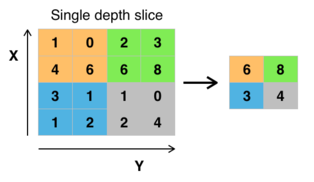
\includegraphics[width=0.5\textwidth]{Figures/4/Max_pooling.png}
\caption{Illustration of the max pooling operation, the function outputs a maximum output in every 2 by 2 square \citep{wiki:Convolutional}}
\label{fig:max}
\end{figure}
 

\subsection{Implementation of a Convolutional Neural Network}

Training a convolutional neural network requires a lot of parallel computing power. Therefore,  GPU cards are used for training convolutional neural networks. Since a computing device with separate GPU unit was not available; it was decided to focus on smaller CNN architectures that could be trained on a CPU.

It was chosen to design a convolutional neural network with three convolutional layers and one fully connected layer. First convolutional layer applies one by one convolution to the input image and creates four convolution images. These convolution images are then passed through an activation function at outputs of this function are passed into a second convolutional layer. Besides convolution, a max pooling operation is also applied in the second and third layers of the network. The final convolutional layer outputs twelve seven by seven convolutional images. These images are passed into the fully connected layer, and finally, the class of an image is calculated in the final layer \autoref{fig:con_mod}



\begin{figure}[h]
\centering
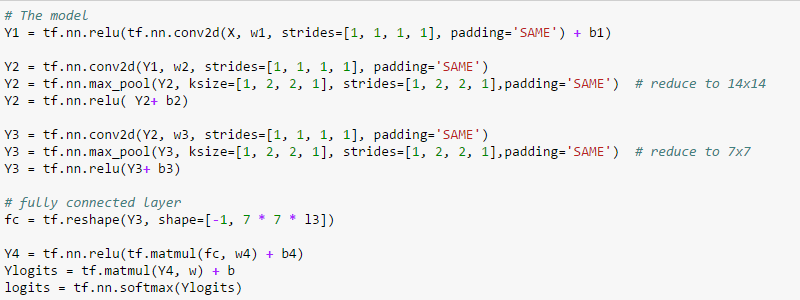
\includegraphics[width=0.5\textwidth]{Figures/4/conv.PNG}
\caption{The convolutional network model in written TensorFlow}
\label{fig:con_mod}
\end{figure}

Firstly, the images of the dataset were resized to 26 by 26 pixels to reduce the dimensionality of the data.
It was unknown how long it would take to train the network, so it was decided to reduce the dimensionality even further by converting images to greyscale.

Then, a convolutional neural network was trained for 100 epochs. The best learning rate that was used in the deep learning network (0.0001) was too small for the convolutional network. The learning rate was gradually increased, and it was observed that learning rate 0.003 suited the network best. The network with this learning rate achieved 100 percent accuracy on the training dataset in 68 epochs. Despite the fact, that the result looked very impressive, it was known that convolutional neural networks tend to overfit the data. That means that they learn to classify the training dataset very accurately but do not classify the test dataset well. Therefore, the classifier was tested on the test dataset. It achieved 38.12 percent accuracy, which was not that good.

The algorithm was modified to accept RGB images, for testing whether colour channels have an influence on the classification accuracy. After the network was trained, it was observed that it achieved 47.51 percent accuracy on the test dataset. More than 9 percent increase in accuracy showed that colour is an important component for a food image classification and should be kept if possible. The architecture of both convolutional neural networks trained is shown in \autoref{table:convi}.

\begin{table}[h]
\begin{center}
 %\setlength\tabcolsep{2pt}
\begin{tabular}{ |c|c|c|c|c| }
\hline
 Input image&Learning Rate &   Number of layers & Architecture & Accuracy \\   \hline
28x28x1 & 0.003   &   5  &  3 x conv, fc, o  & 38.12\% \\
28x28x3 & 0.003   &   5  &  3 x conv, fc, o  & 47.50\% \\
 \hline
\end{tabular}
\caption{Details about the first two convolutional models tried}

\label{table:convi}
\textit{ conv - convolutional layer, fc - fully connecteed layer, o - output layer}
\end{center}
\end{table}

\subsection{Improving the Convolutional Neural Network}

Since both classifiers achieved a hundred percent accuracy on the training dataset and performed poorly on the test dataset, it was clear that the classifiers were overfitting the data. It was decided to add dropout layers to the network, to fix this problem. Dropout is a method used to prevent neural networks from overfitting. The key idea is to randomly drop units (along with their connections) from the neural network during training \cite{dropout}. Dropout function prevents neurons from co-adapting too much. 

50 percent dropout rate was added to the every layer of the network. The Introduced drop layer helped to prevent the network from overfitting. However, because of the high dropout ratio the network was unable to optimise the weights and it classified worse than previously trained models. It was tried to increase the learning rate. This solution did not work because larger step size caused the optimisation algorithm to keep overshooting the minimum. The other tried solution was increasing the probability to keep neuron connections to 80 percent. It improved the classification accuracy for both grayscale and RGB image classification, but the improvement was only marginal (49.04 percent accuracy for RGB test data and 40 percent accuracy for the grayscale image classifier). Lastly, it was tried to keep 90 percent of the neuron connections in the network, but it decreased the accuracy on the test dataset. It was concluded that learning rate 0.003 and 20 percent dropout probability were the best set of hyperparameters for this network. Because there were no more hyperparameters that could be further optimised it was tried to increase the size of input images.


\subsection{CNN on larger images}

It was expected that larger image size would lead to a better accuracy score when performing image classification because larger image sizes allow more information to be preserved in pictures. The network was redesigned to take 56x56x3 pictures as an input. One more convolutional and a max-pooling layer were also introduced to the architecture of the network . It was tried to find the optimal learning rate. The network was trained with 0.003 learning rate and a 20 percent drop probability for 30 epochs. It was noticed that learning rate, which worked very well for the previous neural network, was too high for this network. Because of that, the gradient optimisation algorithm kept overshooting the minimum and training accuracy, and loss stayed the same during the training of the model. To find the optimal learning rate, it was gradually lowered until it reached 0.0015. With this learning rate, the algorithm was able to learn the optimal weights. When tested it achieved 60.72 test accuracy. It was tried to increase the number of epochs to 100 because more epochs meant that the weight could be optimised more correctly. After testing the model on the test dataset, it was observed that the accuracy increased to 62.26 percent.

Finally, it was tested whether modifying the architecture of dropout layers could improve the performance of the classifier. In the previous model, dropout was used in every layer except the fully connected one. The dropout was added to this layer too. However, after adding the dropout, the learning rate value of 0.0015 was too large. After decreasing the value of the learning rate to 0.001, it became possible to train the network. A trained network with 20 percent drop probability reached 69.34 percent accuracy, and a trained network with 30 percent drop probability reached 63.98. Therefore, 20 percent was a better drop rate in both approaches. It was also tried to modify the model to use dropout only in a fully connected layer. Because only one dropout layer was used the dropout probability needed to be increased to 50 percent. The network was trained with a 0.001 learning rate. However, training accuracy of the model improved very slowly. Therefore, learning rate was increased and the optimal its optimal value of 0.002 was found. The trained model was tested on the test data set. The accuracy of the model o the test was 51.54 percent. A table of CNN networks that were constructed for 56x56x3 images can be seen in \autoref{table:53x53}.


\begin{table}[h]
\begin{center}
\begin{tabular}{ |c|c|p{3.3 cm}|p{2 cm}|c|c|} 
 \hline
 Learning Rate & Drop probability & Network layers with drop &Training Epochs&Accuracy \\   \hline
0.001   &   20\%  & Every except fully  connected  & 30 & 57.08\% \\ \hline
0.0015    &   20\%   &  Every  except fully connected  & 30  & 60.72\% \\ \hline
0.0015    &   20\%   &  Every  except fully connected  & 100  & 62.26\% \\ \hline
0.001    &   30\%   &  Every  & 100  & 63.98\% \\ \hline
0.001    &   20\%   &  Every  & 100  & 69.34\% \\ \hline
0.002    &   50\%   &  Fully connected& 100  & 51.54\% \\  \hline
\end{tabular}
\caption{Different configurations for convolutional neural networks tried with 56x56x3 pictures}
\label{table:53x53}
\end{center}
\end{table}



\section{Transfer Learning Technique}

\subsection{What is Transfer Learning}

Currently, all state of the art image classifiers are large convolutional neural networks.  For training these networks, large GPU clusters were used, and it usually took multiple weeks of computing to train these models. For example,  the Google's Inception v3 network was trained on a cluster of  50 computers with  NVidia Kepler GPUs \cite{incept}. It is impossible to train this network using only one computer because the network has millions of parameters that require a massive amount of memory and computation power. The only way how this network could be retrained for a different dataset on a regular computer is by using a transfer learning approach. 

Transfer learning is a technique that shortcuts a lot of this work by taking a fully-trained model for a set of categories like ImageNet and retrains it from the existing weights for new classes \cite{tensorflow}. Usually, only the two final layers of a neural network are retrained to save time. The reason why retraining only the final two layers is effective it that convolutional layers tend to activate to patterns of different shapes, colours and edges. Such patterns appear not to be specific to a particular dataset or task, but can be applicable to many datasets and tasks \cite{transfer}.

It was chosen to retrain the Google's Inception v3 model. A python script for loading and retraining this model is publicly available in the Tensorflow's Github repository \cite{gitretrain}. The script provides the ability to tweak hyperparameters such as a learning rate, number of training epochs and a batch size. 


\begin{figure}[h]
\centering
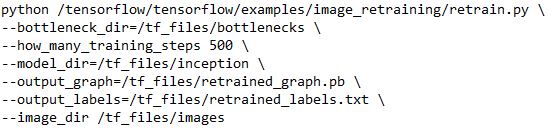
\includegraphics[width=0.5\textwidth]{Figures/4/term.PNG}
\caption{Terminal command used to launch python script that retrains the Inception v3 Model}
\label{fig:retrain}
\end{figure}

\subsection{ Retraining of the Inception v3 Model}

The classifier was retrained with a learning rate = 0.01, a number of epochs = 500 , and a batch size = 100. The script split the dataset to use 80 percent of it as a training set, 10 percent of it as a testing set used to test the classifier after each epoch and the last 10 percent as a validation dataset used to test the trained model. The terminal command that was used to run the retrain.py can be seen in \autoref{fig:retrain}.

When retrain.py was run it firstly calculated bottlenecks for all the images in the dataset. A bottleneck is a term used for naming the layer just before the final output layer that does the classification. Calculation of bottlenecks took a significant amount of time. The script saved the calculated bottlenecks to the disk, so this task was only needed to run once.

After the calculation of the bottlenecks. The weights of the penultimate and final layers were set, and optimisation of weights in these layers began. The training progress of the classifier was shown in the terminal (\autoref{fig:retrain}). It was observed that just after ten epochs the classifier reached 96 percent accuracy.  After running the weight optimisation algorithm for 500 iterations, the final trained model achieved 98.2 percent accuracy when tested on 507 validation samples. That meant that the classifier was able to classify 98 from 100 pictures of unseen food correctly.  This accuracy is much higher than accuracies achieved by every other classifier.

To get a better understanding how can this classifier perform on the real-world data 5 example pictures for each class were downloaded.These images were a had picked examples of each class. The python script that loads the learnt model from disk, and feeds classifier with images from the given folder was written. After running the classification on 20 accumulated images, one classification error was detected. The classifier classified a picture of deep pan pizza \autoref{fig:miss} as fish and chips. It was expected that this example might get misclassified because there were no deep pan pizzas in a training dataset. The smooth structure of a crust of the pizza can also resemble a battered fish. 


\begin{figure}[h]
\centering
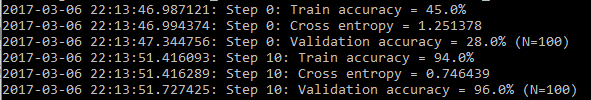
\includegraphics[width=0.5\textwidth]{Figures/4/term-train.PNG}
\caption{Retraining process of the classifier, 96 percent accuracy was reached in just 10 epochs}
\label{fig:retrain-2}
\end{figure}

\begin{figure}[h]
\centering
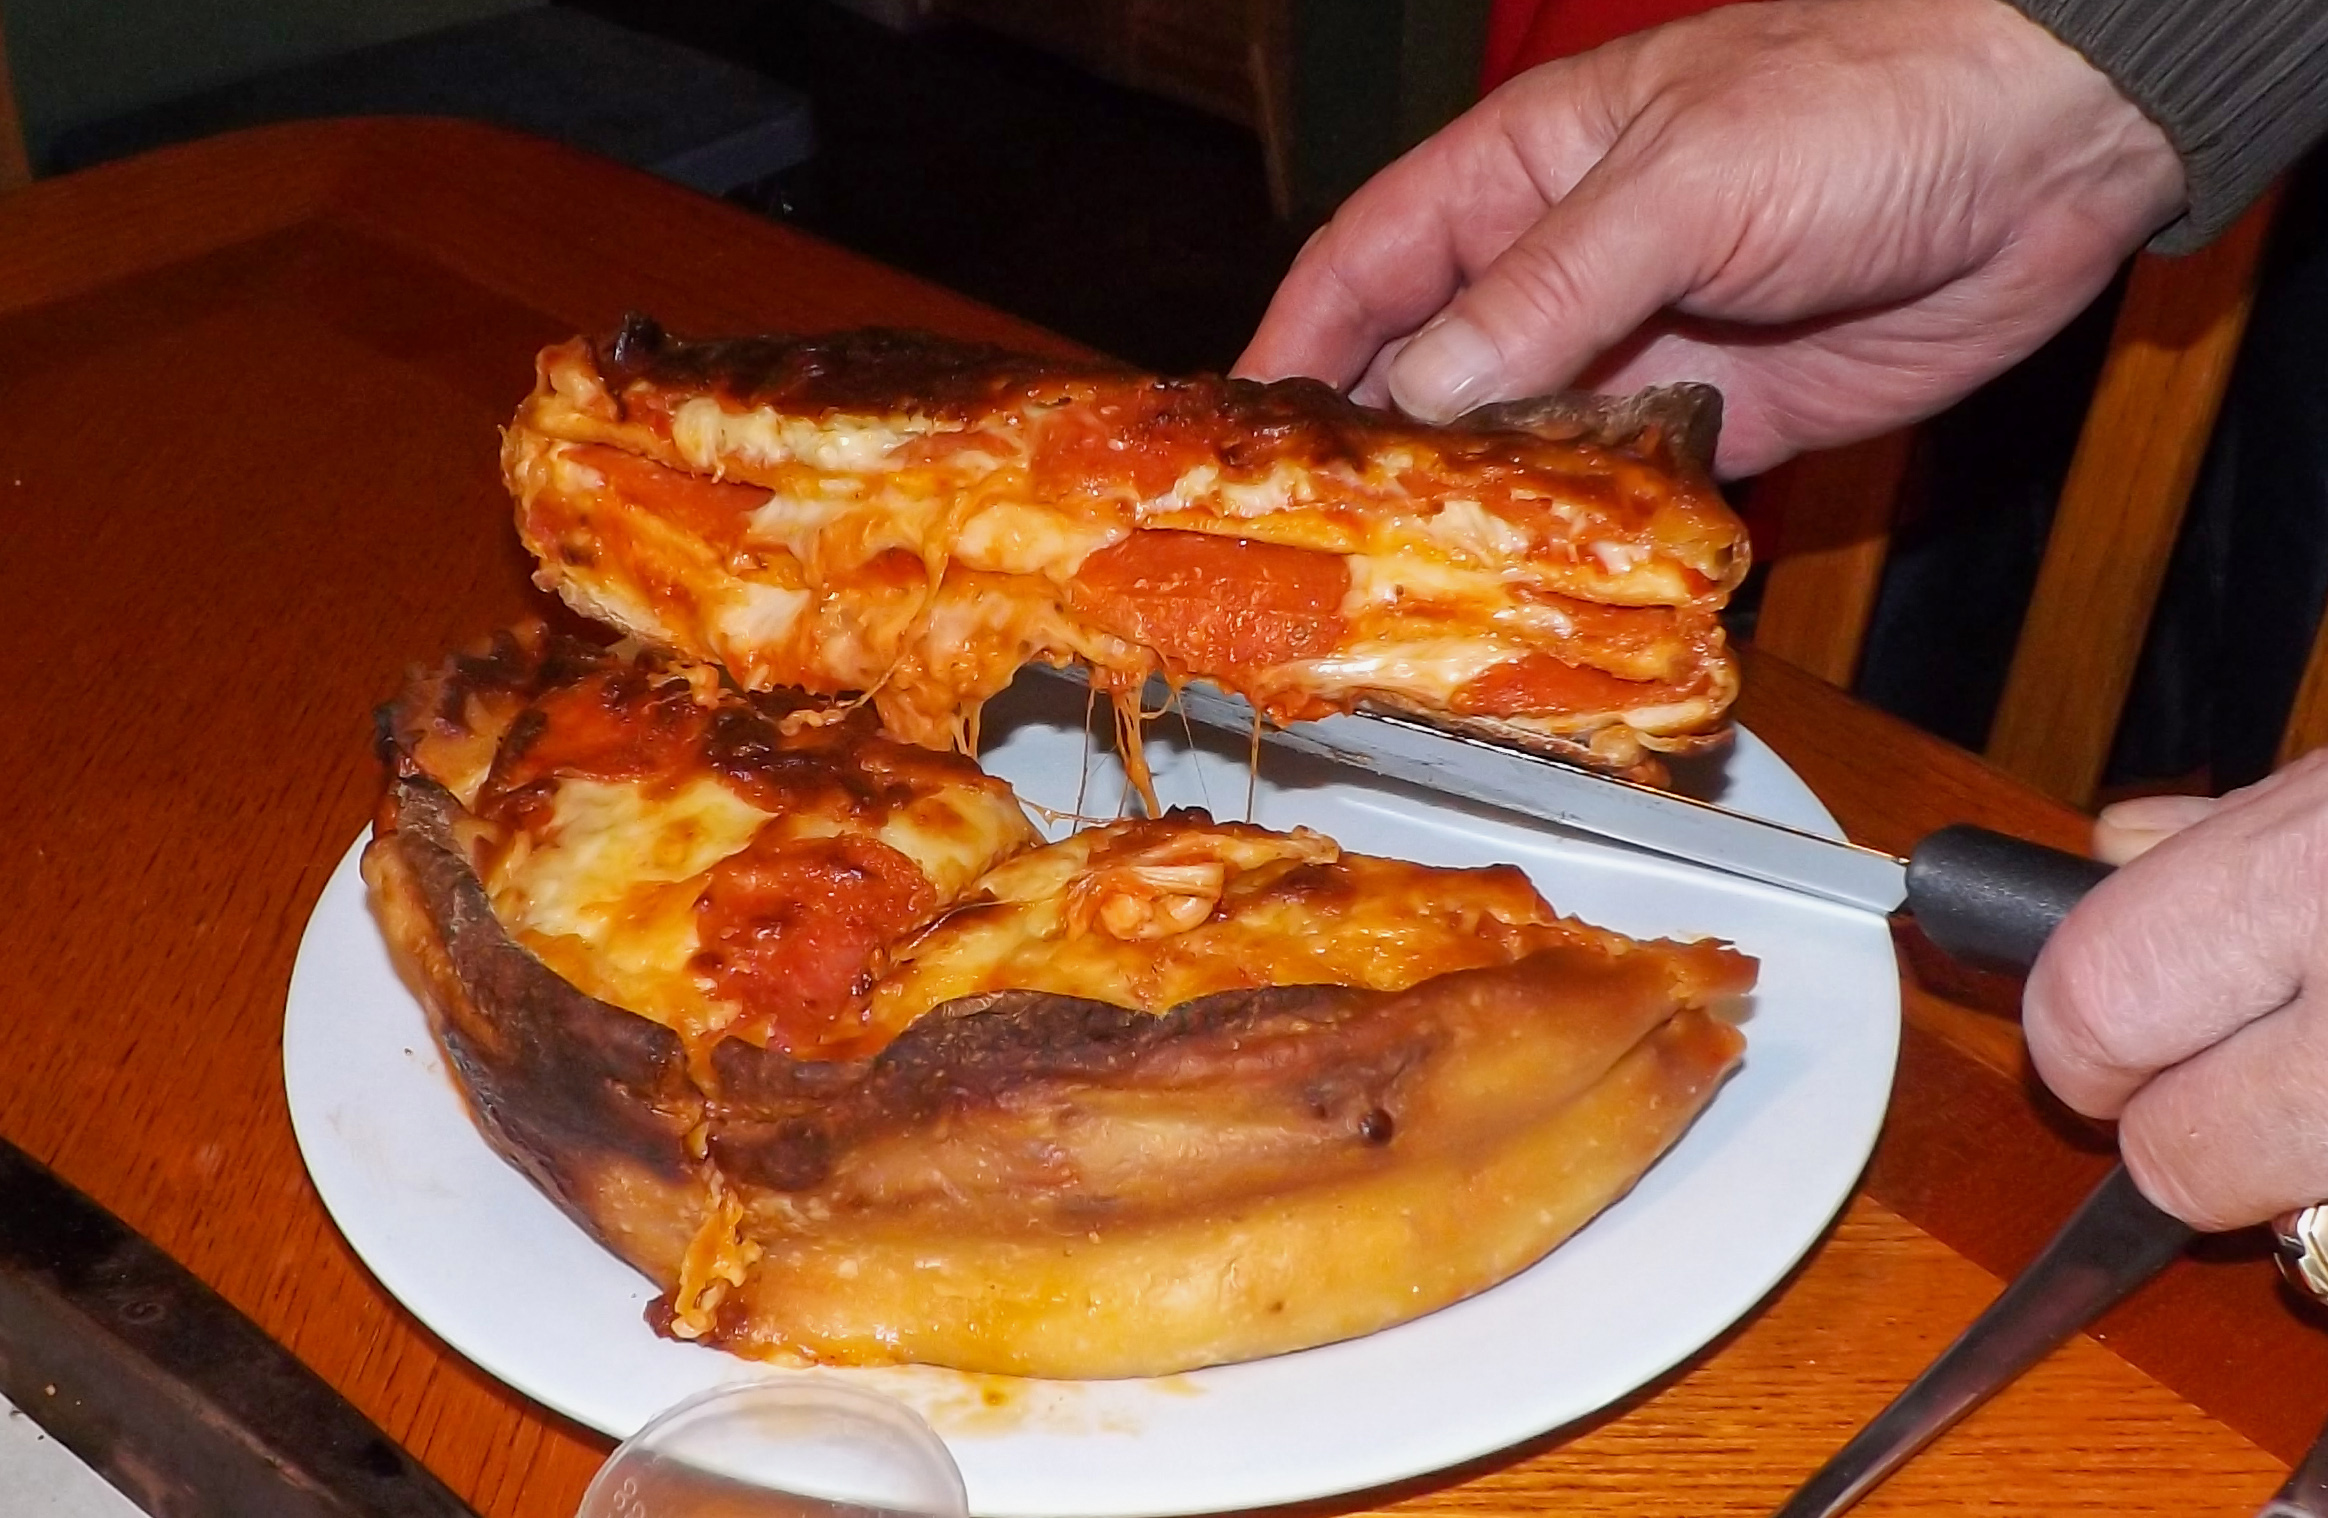
\includegraphics[width=0.5\textwidth]{Figures/4/4.jpg}
\caption{A picture of a deep pan pizza that was missclassified as a fish}
\label{fig:miss}
\end{figure}




\section{Summary}

To conclude, it can be clearly seen that deep learning networks on average performed much better than a standard machine learning models. The accuracy achieved by a transfer learning model was very high. The model could be used in practice, because the error rate is very low.

However, finding the optimal parameters for the deep neural network models are a much harder task. Creating architectures of neural networks take a lot of effort. It can not be known beforehand what structure of the network will work on a particular task. Therefore, many architectures have to be tried to find a suitable architecture. Even then it is unknown if the chosen architecture is actually the best because the configuration space is gigantic.

In the next chapter, the results of all classification methods are going to be compered.